%%
%% This is file `sample-sigconf.tex',
%% generated with the docstrip utility.
%%
%% The original source files were:
%%
%% samples.dtx  (with options: `sigconf')
%% 
%% IMPORTANT NOTICE:
%% 
%% For the copyright see the source file.
%% 
%% Any modified versions of this file must be renamed
%% with new filenames distinct from sample-sigconf.tex.
%% 
%% For distribution of the original source see the terms
%% for copying and modification in the file samples.dtx.
%% 
%% This generated file may be distributed as long as the
%% original source files, as listed above, are part of the
%% same distribution. (The sources need not necessarily be
%% in the same archive or directory.)
%%
%% The first command in your LaTeX source must be the \documentclass command.
\documentclass[sigconf]{acmart}
%% NOTE that a single column version may be required for 
%% submission and peer review. This can be done by changing
%% the \doucmentclass[...]{acmart} in this template to 
%% \documentclass[manuscript,screen]{acmart}
%% 
%% To ensure 100% compatibility, please check the white list of
%% approved LaTeX packages to be used with the Master Article Template at
%% https://www.acm.org/publications/taps/whitelist-of-latex-packages 
%% before creating your document. The white list page provides 
%% information on how to submit additional LaTeX packages for 
%% review and adoption.
%% Fonts used in the template cannot be substituted; margin 
%% adjustments are not allowed.
%%
%%
%% \BibTeX command to typeset BibTeX logo in the docs
\AtBeginDocument{%
  \providecommand\BibTeX{{%
    \normalfont B\kern-0.5em{\scshape i\kern-0.25em b}\kern-0.8em\TeX}}}

%% Rights management information.  This information is sent to you
%% when you complete the rights form.  These commands have SAMPLE
%% values in them; it is your responsibility as an author to replace
%% the commands and values with those provided to you when you
%% complete the rights form.
% \setcopyright{acmcopyright}
% \copyrightyear{2018}
% \acmYear{2018}
% \acmDOI{XXXXXXX.XXXXXXX}

%% These commands are for a PROCEEDINGS abstract or paper.
% \acmConference[Conference acronym 'XX]{Make sure to enter the correct
%   conference title from your rights confirmation emai}{June 03--05,
%   2018}{Woodstock, NY}
% %
% %  Uncomment \acmBooktitle if th title of the proceedings is different
% %  from ``Proceedings of ...''!
% %
% %\acmBooktitle{Woodstock '18: ACM Symposium on Neural Gaze Detection,
% %  June 03--05, 2018, Woodstock, NY} 
% \acmPrice{15.00}
% \acmISBN{978-1-4503-XXXX-X/18/06}


%%
%% Submission ID.
%% Use this when submitting an article to a sponsored event. You'll
%% receive a unique submission ID from the organizers
%% of the event, and this ID should be used as the parameter to this command.
%%\acmSubmissionID{123-A56-BU3}

%%
%% The majority of ACM publications use numbered citations and
%% references.  The command \citestyle{authoryear} switches to the
%% "author year" style.
%%
%% If you are preparing content for an event
%% sponsored by ACM SIGGRAPH, you must use the "author year" style of
%% citations and references.
%% Uncommenting
%% the next command will enable that style.
%%\citestyle{acmauthoryear}

%%
%% end of the preamble, start of the body of the document source.
\begin{document}

%%
%% The "title" command has an optional parameter,
%% allowing the author to define a "short title" to be used in page headers.
\title{CSC 2549 Project: Stable Fluids Implementation}

%%
%% The "author" command and its associated commands are used to define
%% the authors and their affiliations.
%% Of note is the shared affiliation of the first two authors, and the
%% "authornote" and "authornotemark" commands
%% used to denote shared contribution to the research.
\author{Anqi Joyce Yang}
\email{ajyang@cs.toronto.edu}

%%
%% The code below is generated by the tool at http://dl.acm.org/ccs.cfm.
%% Please copy and paste the code instead of the example below.
%%
\begin{CCSXML}
<ccs2012>
 <concept>
  <concept_id>10010520.10010553.10010562</concept_id>
  <concept_desc>Computing methodologies~Animation</concept_desc>
  <concept_significance>500</concept_significance>
 </concept>
%  <concept>
%   <concept_id>10010520.10010575.10010755</concept_id>
%   <concept_desc>Computer systems organization~Redundancy</concept_desc>
%   <concept_significance>300</concept_significance>
%  </concept>
%  <concept>
%   <concept_id>10010520.10010553.10010554</concept_id>
%   <concept_desc>Computer systems organization~Robotics</concept_desc>
%   <concept_significance>100</concept_significance>
%  </concept>
%  <concept>
%   <concept_id>10003033.10003083.10003095</concept_id>
%   <concept_desc>Networks~Network reliability</concept_desc>
%   <concept_significance>100</concept_significance>
%  </concept>
</ccs2012>
\end{CCSXML}

\ccsdesc[500]{Computing methodologies~Animation}
% \ccsdesc[500]{Computer systems organization~Embedded systems}
% \ccsdesc[300]{Computer systems organization~Redundancy}
% \ccsdesc{Computer systems organization~Robotics}
% \ccsdesc[100]{Networks~Network reliability}

%%
%% Keywords. The author(s) should pick words that accurately describe
%% the work being presented. Separate the keywords with commas.
\keywords{stable fluids, Navier-Stokes, Python, fluid simulation, stable solver}

%% A "teaser" image appears between the author and affiliation
%% information and the body of the document, and typically spans the
%% page.
% \begin{teaserfigure}
%   \includegraphics[width=\textwidth]{sampleteaser}
%   \caption{Seattle Mariners at Spring Training, 2010.}
%   \Description{Enjoying the baseball game from the third-base
%   seats. Ichiro Suzuki preparing to bat.}
%   \label{fig:teaser}
% \end{teaserfigure}

%%
%% This command processes the author and affiliation and title
%% information and builds the first part of the formatted document.
\maketitle

\section{Introduction}
From water to smoke to air, fluids are an indispensible part of our lives, and
fluid simulation has been widely studied in computer graphics. In this project,
we implement Jos Stam's 1999 paper on Stable Fluids~\cite{Stam1999Fluid}, which
presents a stable Navier-Stokes solver that simulates gaseous-like phenomena.
One key strength of the paper is that it proposes a novel advection approach
that enables large time steps for faster simulation.

This project implements the stable fluids solver in Python for both 2D and 3D fluid fields.
The rest of this report will be divided as follows: Section~\ref{sec:related}
discusses related works and resources that have been used to understand the paper.
Section~\ref{sec:algo} goes over the stable fluids solver presented in the original
paper~\cite{Stam1999Fluid}. Section~\ref{sec:impl} details our implementation and
modifications to the original algorithm. Finally, Section~\ref{sec:result} showcases
some qualitative results.

\section{Related Work}
\label{sec:related}
To better understand the Stable Fluids paper~\cite{Stam1999Fluid} that we are implementing, we have consulted multiple resources, including Bridson's 2008 Fluid Simulation textbook~\cite{Bridon2008FluidBook}, Professor David Levin's fluid simulation lecture video~\cite{csc417fluidvideo}, Dan Piponi's fluid simulation talk~\cite{piponitalk}, and Philip Zucker's blog post~\cite{zuckerblog}.

\section{Algorithm}
In this section, we describe the core stable fluid simulation algorithm introduced in~\cite{Stam1999Fluid}. Note that we mostly follow the notations used in the paper for consistency and clarity, with the exception that the paper uses $a$ for scalar values and $S$ as external source while we use $S$ and $P$ respectively, and that the paper uses time step as a continuous value (the new time step is $t + \Delta t$), while we use time step as a discrete value (the new time step is $t + 1$ at time $\Delta t$ later).
\label{sec:algo}
\subsection{Problem Setting}
Given a two-dimensional fluid field with spatial coordinates $\mathbf{x} = (x, y)$ or a three-dimensional field with coordinates $\mathbf{x} = (x, y, z)$, we can define the velocity field $\mathbf{u}$, the pressure field $p$, and the scalar field $S$, where $\mathbf{u}(\mathbf{x}, t)$ corresponds to the two-dimensional or three-dimensional velocity, $p(\mathbf{x}, t)$ represents the pressure, and scalar quantities $S(\mathbf{x}, t)$ represent additional information such as colors or temperature at position $\mathbf{x}$ and time step $t$.

From time step $t$ to time step $t + 1$ with change of time $\Delta t$, following the Navier-Stokes equation, the velocities and pressure in the fluid field will change according to the external force $\mathbf{f}(\mathbf{x}, t)$ applied, the density $\rho$ and the kinematic viscosity $\nu$ of the liquid. In addition, the substances $S$ will change according to the updated velocities, the diffusion constant $\kappa$ of the scalar values and the dissipation rate $\alpha$. We next describe the Navier-Stokes equation and the specifics of how to update these quantities in a fluid field.

% Given an input grid of dimension either 2 or 3, the stable fluids algorithm solves
% for velocities and scalar values (such as textures or temperature) located at the
% cell centers. Following the Navier-Stokes equation, the solver divides the velocity
% update in four steps: (1) add forces, (2) transport/advection, (3) diffusion, and
% (4) projection (such that the velocities are divergence-free). In addition,
% the scalar fields can also be solved in four steps: (1) add forces, (2) transport/advection,
% (3) diffusion, and (4) dissipation.
% In order to allow for large time steps, in the advection step, the author
% introduces a semi-Lagragian approach~\cite{Bridon2008FluidBook} to update quantities
\subsection{The Navier-Stokes Equation}
The Navier-Stokes equation states that the change in velocities $\mathbf{u}$ and the pressure $p$ should satisfy the following constraints:
\begin{equation}
\label{eq:stokes}
\begin{split}
  &\frac{\partial \mathbf{u}}{\partial t} = -\nabla\mathbf{u} \cdot \mathbf{u} - \frac{1}{\rho}\nabla p + \nu\nabla^2\mathbf{u} + \mathbf{f}\\
  &\nabla\cdot\mathbf{u} = 0,
\end{split}
\end{equation}
where $\nabla\mathbf{u}$ is the material derivative matrix, $\cdot$ is the matrix product, $\nabla^2 = \nabla\cdot\nabla$ is the laplacian operator, and $\nabla\cdot\mathbf{u}$ is the divergence of the velocities $\mathbf{u}$. Here we assume that the liquid is incompressible, hence the divergence-free $\nabla\cdot\mathbf{u} = 0$ constraint.

\subsection{Stable Fluids Solver}
To update the velocities and pressure at time step $t$ according to the Navier-Stokes equation, we can break down the update process (the right-hand side of Eq.~\ref{eq:stokes}) into 4 steps. Namely, we add the external force, perform advection, diffuse according to the viscosity, and project the velocities to be divergence-free. We next describe each step in detail.

\paragraph{Add force} Given the velocity $\mathbf{w}_0(\mathbf{x}) = \mathbf{u}(\mathbf{x}, t)$ at the previous time step $t$, our goal is to find the updated velocity at time step $t + 1$ which is $\Delta t$ later. First, we apply the external force to derive the updated velocity $\mathbf{w}_1(\mathbf{x})$:
\begin{equation}
  \mathbf{w}_1(\mathbf{x}) = \mathbf{w}_0(\mathbf{x}) + \Delta t \mathbf{f}(\mathbf{x}, t).
\end{equation}
This corresponds to the $\frac{\partial \mathbf{u}}{\partial t} = \mathbf{f}$ part of Eq.~\ref{eq:stokes}.

\paragraph{Advection} Next, we wish to apply the update for $\frac{\partial \mathbf{u}}{\partial t} = -\nabla\mathbf{u} \cdot \mathbf{u}$, which updates the velocities according to the motion in the field. In the Stable Fluids paper, to allow for large time step updates, the author proposed the following technique:
\begin{equation}
  \mathbf{w}_2(\mathbf{x}) = \mathbf{w}_1(\mathbf{p}(\mathbf{x}, -\Delta t)).
\end{equation}
In the Lagrangian view, if a particle moves from location $\mathbf{p}(\mathbf{x}, -\Delta t)$ to $\mathbf{x}$, its velocity should not change. As a result, in the Eulerian view, we can find the velocity at time step $t+1$ at position $\mathbf{x}$ by extracting the velocities at its previous location at time $\Delta t$ ago. This approach is unconditionally stable since the updated velocities always come from the velocities in the previous time step, so the maximum of the new velocity field will never exceed the maximum of the previous velocities. To find the previous location $\mathbf{p}(\mathbf{x}, -\Delta t)$, we use a simple second-order Runge-Kutta method:
\begin{verbatim}
  x_midpoint = x - 0.5 * dt * w1(x)
  p(x, -dt) = x - dt * w1(x_midpoint)
\end{verbatim}

\paragraph{Diffusion} The diffusion step corresponds to the $\frac{\partial \mathbf{u}}{\partial t} = \nu\nabla^2\mathbf{u}$ part of Eq.~\ref{eq:stokes}. We use an implicit method to allow for stability when the viscosity is large:
\begin{equation}
  (\mathbf{I} - \nu\Delta t\nabla^2)\mathbf{w}_3(\mathbf{x}) = \mathbf{w}_2(\mathbf{x}),
\end{equation}
where $\mathbf{I}$ is the identity matrix.

\paragraph{Projection} Finally, to solve for the pressure $\frac{\partial \mathbf{u}}{\partial t} = -\frac{1}{\rho}\nabla p$ while ensuring that the velocities are divergence free, we can apply the divergence operator on both sides:
\begin{equation}
  \nabla\cdot\mathbf{w}_4(\mathbf{x}) = \nabla\cdot\mathbf{w}_3(\mathbf{x}) - \frac{\Delta t}{\rho}\nabla\cdot\nabla p(\mathbf{x}) = 0
\end{equation}
This gives us
\begin{equation}
\begin{split}
  &\nabla^2 p(\mathbf{x}) = \frac{\rho}{\Delta t}\nabla\cdot\mathbf{w}_3(\mathbf{x})\\
  &\mathbf{w}_4(\mathbf{x}) = \mathbf{w}_3(\mathbf{x}) - \frac{\Delta t}{\rho}\nabla p(\mathbf{x})
\end{split}
\end{equation}
so that we can solve for the pressure $p$ in the first step, and update the velocities in the second step. The updated velocities $\mathbf{u}(\mathbf{x}, t + 1)$ at the new time step $t + 1$ will thus be $\mathbf{w}_4(\mathbf{x})$.

The scalar value update follows the equation below:
\begin{equation}
  \frac{\partial S}{\partial t} = -\mathbf{u}\cdot\nabla S + \kappa\nabla^2 S - \alpha S + P,
\end{equation}
which accounts for diffusion with constant $\kappa$, dissipation with rate $\alpha$, and an external source term $P$.
Updating the scalar quantities $S(\mathbf{x})$ is similar to the velocity update, except that in the fourth step, we apply dissipation instead of pressure projection:
\begin{equation}
  (1 + \Delta t \alpha)S(\mathbf{x}, t + 1) = S(\mathbf{x}, t).
\end{equation}

\subsection{Boundary Conditions}
We consider two types of boundary conditions. In the fixed boundary condition, we force the velocities at the boundary to be a fixed value (\emph{e.g., 0}). In the periodic boundary condition, the fluid has no boundaries and wraps around. The paper proposes a Fourier-based approach to handle the periodic boundary condition, while in our implementation we can simply encode the wrapping effect when constructing the divergence operator. See Sec.~\ref{sec:impl} for more details.

\section{Implementation}
\label{sec:impl}
\subsection{Discretization}
% Given a two-dimensional fluid grid of size $N_1\times N_2$ with spatial coordinates $\mathbf{x} = \{(x, y)\}$ or a
% three-dimensional grid of size ${N_1 \times N_2 \times N_3}$ with coordinates $\mathbf{x} = \{(x, y, z)\}$,
% we can define a velocity field $\mathbf{u}$ \in $\mathbb{R}^{N_1\times N_2 \times 2}$ in
% two dimension or $\mathbf{u}$ \in $\mathbb{R}^{N_1\times N_2 \times N_3 \times 3}$ in three
% dimension, where each velocity $u_{i,j}$ (or $u_{i,j,k}$ in 3D) is located at the center of the
% cell $x_{i,j}$ (or $x_{i,j,k}$ respectively). Similarly, we can define a scalar field $S \in \mathbb{R}^{N_1\times N_2}$ (2D) and $\mathbb{R}^{N_1\times N_2 \times N_3}$ (3D) consisting
% scalar values such as colors or temperature corresponding to the input grid.

% Additionally, the grid has an underlying pressure field $p$. Then, at each time step $t + 1$, the quantities on the velocity field $\mathbf{u}$, the scalar field $S$ and the pressure field $p$ will change due to the movement of the fluid. Specifically, the values will get updated according to the change of time $\Delta t$ from the previous time step, the external force defined by a force field $\mathbf{f}$

Following the paper, we descretize the spatial coordinates of the fluid field $\mathbf{x}$ as a two-dimensional $N_1\times N_2$ grid or a three-dimensional $N_1\times N_2 \times N_3$ grid. The velocities $\mathbf{u} \in \mathbb{R}^{N_1\times N_2 \times 2}$ (or $\mathbb{R}^{N_1\times N_2 \times N_3 \times 3}$ in 3D) lie on the center of each cell. Similarly, the scalar fields $S \in \mathbb{R}^{N_1\times N_2 \times C}$ (or $\mathbb{R}^{N_1\times N_2 \times N_3 \times C}$ in 3D) where $C$ is the number of channels (\emph{e.g.}, $C = 3$ for an RGB color field) are also defined at cell centers. For simplicity, we assume two-dimensional grid in the rest of this section.

The advection step computes a previous location $\mathbf{p}(\mathbf{x}, -\Delta t)$, which is in the continuous coordinate domain. To extract the velocities and scalar quantities at this location, we apply a second-order interpolation over the velocity and scalar fields.

To construct the laplacian operator $\nabla^2$ during the diffusion stage, we use a finite difference approach to precompute a $(N_1\times N_2)\times(N_1\times N_2)$ laplacian matrix at cell centers. For the pressure projection stage, we employ a staggered Marker-and-Cell (MAC) grid~\cite{harlow1965MAC}. Specifically, we construct a staggered MAC grid of size $(N_1 - 1)\times(N_2 - 1)$ where each staggered cell center corresponds to a corner in the collocated cell. We transfer the velocities from the collocated grid to the edges/faces of a staggered MAC grid, solve for pressure at cell center with sparse solvers, and then transfer the updated velocities back to the original cell-centered collocated grid.

\subsection{Implementation Details}
We implement the stable fluids solver in Python for both 2D and 3D applications. We use the sparse solvers provided by \texttt{scipy}~\cite{scipy} to solve the sparse linear equations in diffusion and pressure solve. We additionally employ the \texttt{scipy.ndimage} function for interpolation during advection. For the periodic boundary condition, we use the \texttt{wrap} mode for both velocity and scalar interpolation. For the fixed boundary condition, we set the velocity at boundary to 0, and use the \texttt{constant} mode for velocity interpolation and the \texttt{nearest} mode for the scalar field interpolation.

\subsection{Modifications}
Our implementation differs from the original algorithm outlined in~\cite{Stam1999Fluid} in three major ways.

First, for pressure solve, the paper uses the FISHPAK library to solve on the collocated grid. Since the FISHPAK library is not available in Python, and the staggered Marker-and-Cell (MAC) grid~\cite{harlow1965MAC} (which places velocities on the edges/faces and pressure at the center) is a popular choice for pressure solve in fluid simulation nowadays~\cite{Foster95realisticanimation, fluidcoupling07, variationalstokes2017, csc417fluidvideo}, we replace the original implementation with a staggered MAC grid combined with sparse solvers from the Python \texttt{scipy} library~\cite{scipy}.

Second, at each time step iteration, the original paper updates velocities and scalar quantities in two separate passes (\emph{i.e.}, \texttt{VStep} and \texttt{SStep}). It first computes the new velocities \texttt{U1} at time step $t + 1$, and then uses the new velocities \texttt{U1} to update the scalar field during advection. As a result, in the same iteration, the velocity field and the scalar field are advected with two different velocities (\texttt{U0} vs. \texttt{U1}). In our implementation, we merge the \texttt{VStep} and \texttt{SStep} such that the velocities and the scalar field are both updated with the previous velocity $\texttt{U0}$ at time step $t$.

Third, for the periodic boundary condition, instead of using the Fourier transform, we encode the wrapping condition when computing the divergence operators. Specifically, we increase the MAC grid size by one in each dimension, where these new added cells are made up of faces/edges coming from the existing velocity boundaries. As a result, the total number of velocity variables stay the same but we can solve for the additional pressure between the wrapped-around boundaries. 

\section{Results}
\label{sec:result}

\begin{figure}
    \centering
    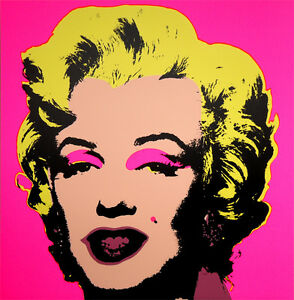
\includegraphics[width=0.32\linewidth]{figs/monroe.jpeg}
    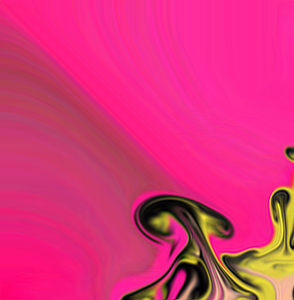
\includegraphics[width=0.32\linewidth]{figs/monroe_fixed.png}
    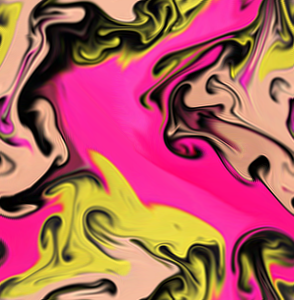
\includegraphics[width=0.32\linewidth]{figs/monroe_periodic.png}
    \caption{Qualitative results for various boundary conditions. (Left) Original image. (Middle) Qualitative result after 300 time steps with fixed boundary condition. (Right) Qualitative result after 300 time steps with periodic boundary condition.
    \label{fig:boundary-condition}}
\end{figure}

\begin{figure}
    \centering
    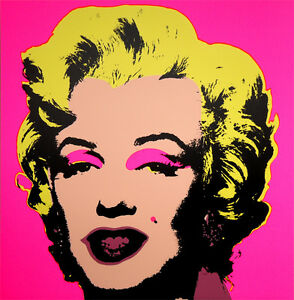
\includegraphics[width=0.32\linewidth]{figs/monroe.jpeg}
    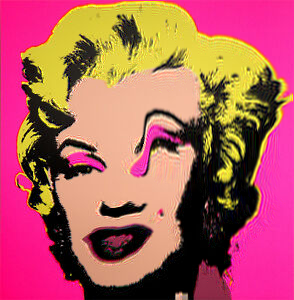
\includegraphics[width=0.32\linewidth]{figs/monroe_vis0.png}
    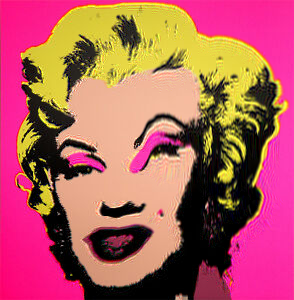
\includegraphics[width=0.32\linewidth]{figs/monroe_vis10.png}
    \caption{Qualitative results for various viscosity results. (Left) Original image. (Middle) Qualitative result after 300 time steps with viscosity $\nu = 0$. (Right) Qualitative result after 300 time steps with viscosity $\nu = 10.0$.
    \label{fig:monroe-vis}}
\end{figure}

\begin{figure}
    \centering
    
\includegraphics[width=0.32\linewidth]{figs/panda_small.jpeg}
    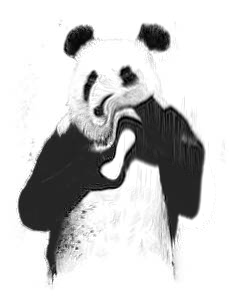
\includegraphics[width=0.32\linewidth]{figs/panda_vis0.png}
    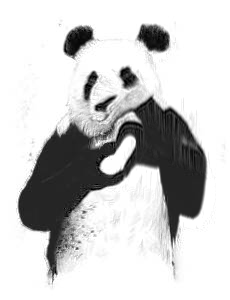
\includegraphics[width=0.32\linewidth]{figs/panda_vis10.png}
    \caption{Qualitative results for various viscosity results. (Left) Original image. (Middle) Qualitative result after 300 time steps with viscosity $\nu = 0$. (Right) Qualitative result after 300 time steps with viscosity $\nu = 10.0$.
    \label{fig:panda-vis}}
\end{figure}

\begin{figure}
    \centering
    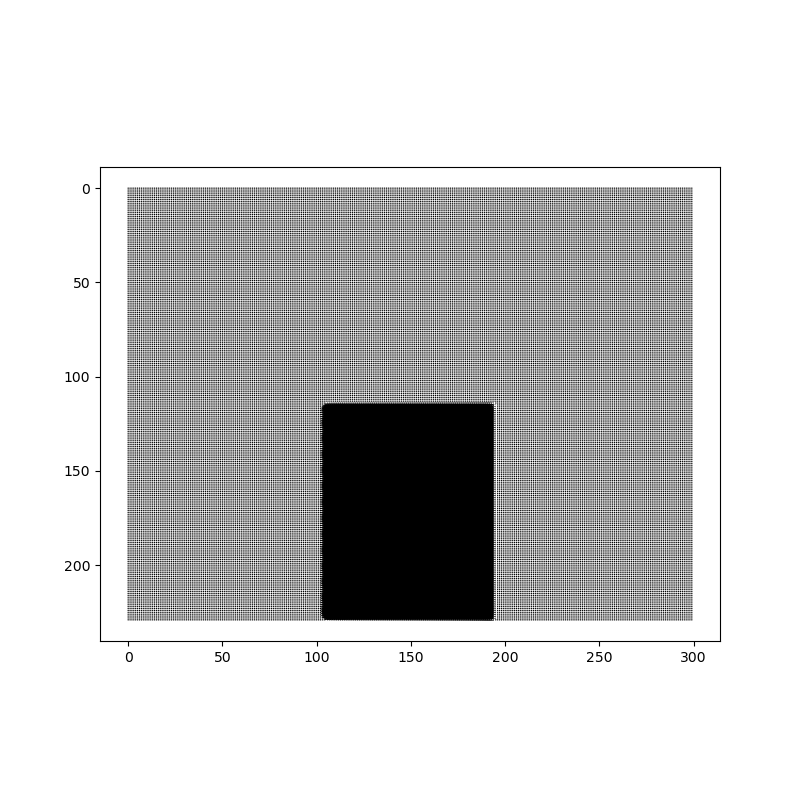
\includegraphics[width=0.32\linewidth]{figs/panda_vis_init_vel.png}
    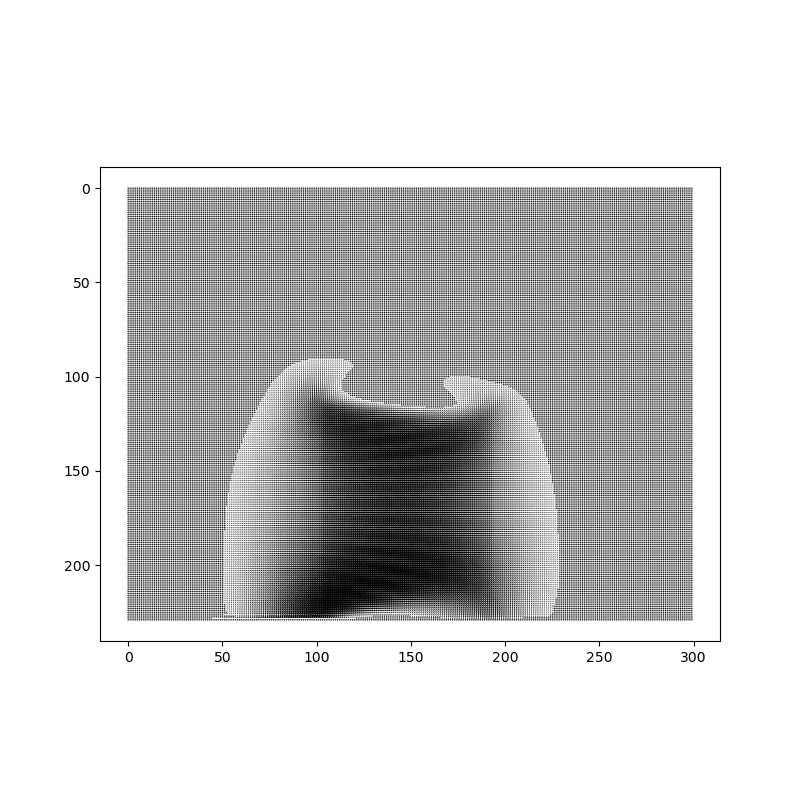
\includegraphics[width=0.32\linewidth]{figs/panda_vis0_vel.png}
    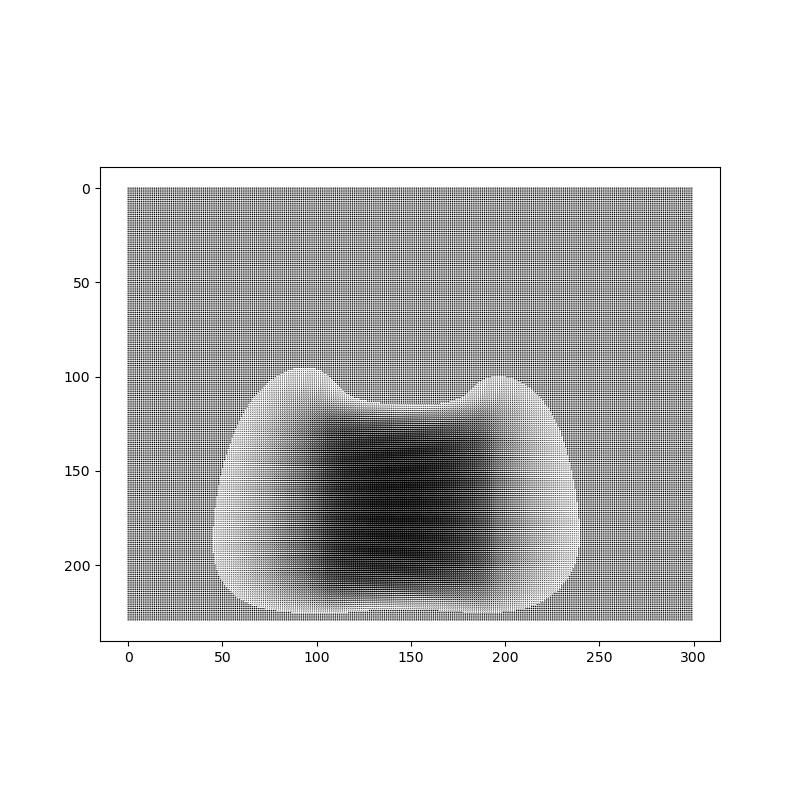
\includegraphics[width=0.32\linewidth]{figs/panda_vis10_vel.png}
    \caption{Velocity plots results for various viscosity results with the fixed boundary condition and constant force applied to the center bottom block at every time step. (Left) Initial velocity. (Middle) Velocity plot after 300 time steps with viscosity $\nu = 0$. (Right) Velocity after 300 time steps with viscosity $\nu = 10.0$.
    \label{fig:panda-vis-vel}}
\end{figure}

\begin{figure}
    \centering
    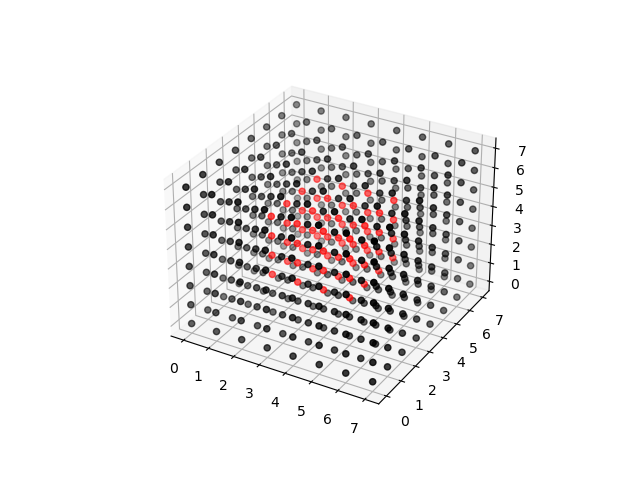
\includegraphics[width=0.49\linewidth]{figs/3d_center_init.png}
    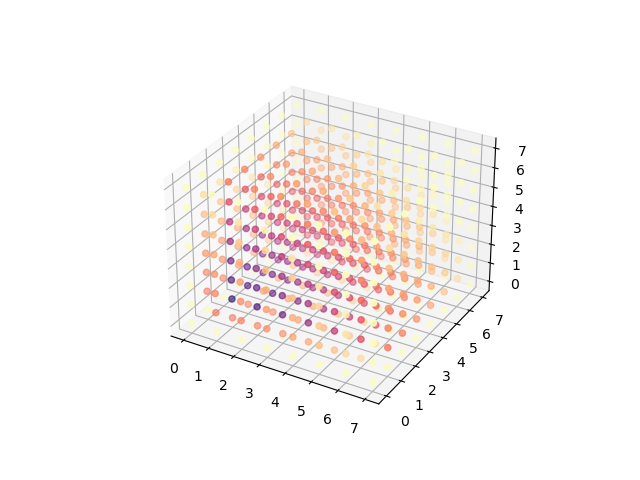
\includegraphics[width=0.49\linewidth]{figs/3d_pretty_init.png}
    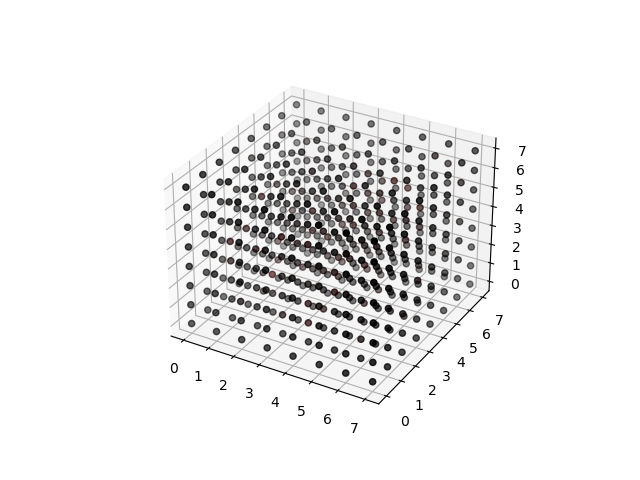
\includegraphics[width=0.49\linewidth]{figs/3d_center_end.png}
    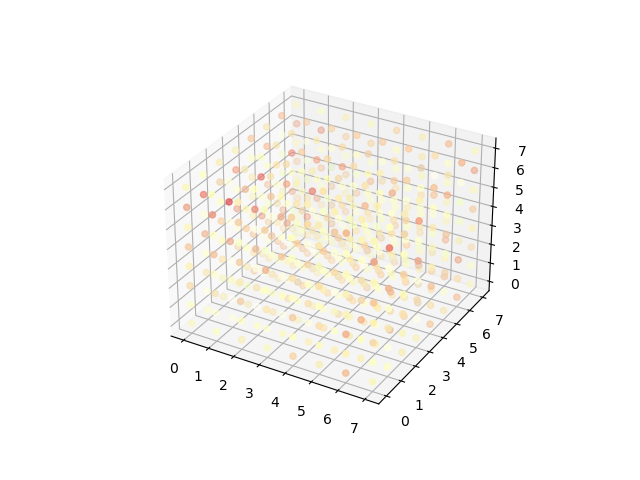
\includegraphics[width=0.49\linewidth]{figs/3d_pretty_end.png}
    \caption{Example visualizations of the 3D application. (Top row) Initialization of two examples. (Bottom row) Qualitative results after 300 iterations.
    \label{fig:3d-vis}}
\end{figure}

We run our solver for both 2D and 3D applications. In this section we show some qualitative results. For more results, please refer to the video\footnote{\url{https://youtu.be/DIZUKA8GSEc}}.

For the 2D application, we run the solver on an input image and create different visual ``melting" effects with various settings (\emph{e.g.}, various external force updates, boundary conditions, viscosity values, etc.).
\paragraph{Boundary Conditions} Fig.~\ref{fig:boundary-condition} showcases results after 300 time steps with the fixed and periodic boundary conditions, where with fixed boundary the colors disappear into the boundary and with periodic boundary condition the texture wraps around.

\paragraph{Kinematic Viscosity} Fig.~\ref{fig:monroe-vis} showcases qualitative results with different kinematic viscosity constants. Note that lower viscosity leads to freer movement. Fig.~\ref{fig:panda-vis} is another qualitative comparison, while Fig.~\ref{fig:panda-vis-vel} illustrates the velocity field.

For more qualitative results with respect to the scalar field diffusion constant and dissipation rate, please refer to the supplementary video. 

For the 3D application, we construct a toy $8\times 8\times 8$ voxel grid, and visualize the updates by plotting the voxel colors with a scatter plot. Please refer to Fig.~\ref{fig:3d-vis} for some qualitative examples. Note that due to time constraint, we did not properly implement both the fixed and periodic boundary conditions in the 3D case. However, we believe that our 2D implementation could be easily refactored and extended into the 3D implementation.

\bibliographystyle{ACM-Reference-Format}
\bibliography{sample-base}

\end{document}
\endinput
%%
%% End of file `sample-sigconf.tex'.
